% Beamer do material do curso de Verão (2015) do IME-USP
% Introdução ao Projeto de Jogos
%
% Baseado no template LaTeX das apresentações do LIDET versão 2
% (https://github.com/luigivieira/LIDET)
%

\providecommand\classopts{}
\expandafter\documentclass\expandafter[table, usenames, svgnames, dvipsnames,%
                                       \classopts]{beamer}
\usepackage{etex}
\usepackage{beamerthemeshadow}
\usepackage[portuguese]{babel}
\usepackage[utf8]{inputenc}
\usepackage[absolute,overlay]{textpos}
\usepackage{array}
\usepackage{framed}
\usepackage{booktabs}
\usepackage[compatibility=false]{caption}
\usepackage{subcaption}
\usepackage{outlines}
\usepackage{ulem}
\usepackage{xcolor,colortbl}
\usepackage{ragged2e}
\usepackage{tikz}
\usepackage{multicol}

% ---------------------------------------------------------------------------- %
% Presentation definitions
% ---------------------------------------------------------------------------- %
\usetheme{Luebeck}
\hypersetup{pdfpagemode=FullScreen} % Starts the presentation in full screen

% layout
\setbeamerfont{frametitle}{size=\normalsize}
\setbeamerfont{title}{size=\normalsize}
\beamertemplatenavigationsymbolsempty
\setbeamertemplate{bibliography item}[text]%
\setbeamertemplate{headline}{} % Remove a barra superior.

% colors
\definecolor{lidet_orange}{rgb}{0.9, 0.49, 0.09}
\definecolor{lidet_black}{rgb}{0.2, 0.2, 0.2}

\setbeamercolor{title}{bg=lidet_orange}
\setbeamercolor{structure}{bg=white, fg=lidet_orange}
\setbeamercolor{normal text}{fg=black}
\setbeamercolor{section in head/foot}{fg=white, bg=lidet_black}
\setbeamercolor{postit}{fg=white, bg=lidet_orange!90!lidet_black}

% shadow
\makeatletter
\pgfdeclareverticalshading[black,bg]{bmb@shadow}{200cm}{%
    color(0bp)=(lidet_black!25);%
    color(4bp)=(black!50!bg);%
    color(8bp)=(black!50!bg)%
}
\pgfdeclareradialshading[black,bg]{bmb@shadowball}{\pgfpointorigin}{%
    color(0bp)=(black!50!bg); color(4bp)=(lidet_black!25)%
}
\pgfdeclareradialshading[black,bg]{bmb@shadowballlarge}{\pgfpointorigin}{%
    color(0bp)=(black!50!bg);%
    color(4bp)=(black!50!bg);%
    color(8bp)=(lidet_black!25)%
}
\makeatother

% Captions for images and tables
\setlength{\abovecaptionskip}{5pt plus 5pt minus 5pt}
\setlength{\belowcaptionskip}{5pt plus 5pt minus 5pt}
\captionsetup[figure]{font=scriptsize,labelfont=scriptsize}
\captionsetup[table]{font=scriptsize,labelfont=scriptsize}
\captionsetup{labelformat=empty,labelsep=none}

% Dimensions for table rules
\setlength\heavyrulewidth{0.1em} 
\setlength\lightrulewidth{0.01em}
\setlength\belowrulesep{0.10ex}
\setlength\aboverulesep{0.10ex}

% Define macros to mark the begining and ending of references
% Basically, handles the automatically spanned frames (due to parameter
% allowframebreaks)
% as backup frames, so they do not influence in the frame numbering
\newcommand{\referencesbegin}{
   \newcounter{framenumberappendix}
   \setcounter{framenumberappendix}{\value{framenumber}}
}
\newcommand{\referencesend}{
   \addtocounter{framenumberappendix}{-\value{framenumber}}
   \addtocounter{framenumber}{\value{framenumberappendix}} 
}

% Adjust footnotes to not overlap the footbar
\addtobeamertemplate{footnote}{}{\vspace{1.0ex}}
\let\oldfootnotesize\footnotesize
\renewcommand*{\footnotesize}{\oldfootnotesize\tiny}

% Redefine the quote environment so short quotes are not broken easily
\renewenvironment{quote}
	{\list{}{\leftmargin1em\rightmargin\leftmargin}%
	\item\relax}
	{\endlist}

% Section frames (that appear before each section)
\AtBeginSection[] 
{
	{
        % Hide the footline locally for these frames
		\setbeamertemplate{footline}{}
		\begin{frame}<beamer>[noframenumbering]
			\begin{center}
				\begin{tikzpicture}
					\node[align=left, left color=lidet_orange,%
                          right color=lidet_orange, draw, rounded corners,%
                          minimum width=10cm, minimum height=1cm]%
                          {\color{white} \textbf{\insertsectionhead}};
				\end{tikzpicture}
			\end{center}
			\footnotesize{\tableofcontents[currentsection,%
                          hideothersubsections]}
		\end{frame}
	}
}

\AtBeginSubsection[]
{
    \begin{frame}
        \centering
        \Large
        \textbf{\insertsubsection}
    \end{frame}
}

\AtBeginSubsubsection[]
{
    \begin{frame}
        \centering
        \large
        \insertsubsection
        \vskip 1em
        \Large
        \textbf{\insertsubsubsection}
    \end{frame}
}

\DeclareGraphicsExtensions{.pdf,.jpg,.png}
\graphicspath{{./images/}}

% ---------------------------------------------------------------------------- %
% Presentation title, author and institution
% ---------------------------------------------------------------------------- %
\newcommand{\lessontitle}{Aula 2 - Pensando na Documentação e\\
                          Regras do Jogo}
\title{\textbf{Introdução ao Projeto de Jogos}}
\subtitle{{\small \lessontitle}}

\newcommand{\autores}{Luiz C. Vieira, Vinícius K. Daros}
\author[\autores]{\scriptsize
    Luiz Carlos Vieira e Vinícius Kiwi Daros\\
    \{luigivieira,vinicius.k.daros\}@gmail.com
}

\newcommand{\lidet}{LIDET (IME - USP)}
\institute[\lidet]{\\[1.0mm] 
Curso de Verão (2015)\\
Departamento de Ciência da Computação}

\date{{\tiny 13 de Janeiro de 2015}}

% ---------------------------------------------------------------------------- %
% Presentation content
% ---------------------------------------------------------------------------- %

% ---------------------------------------------------------------------------- %
\begin{document}
% ---------------------------------------------------------------------------- %

% ---------------------------------------------------------------------------- %
% First Slide (index 0) = cover
% ---------------------------------------------------------------------------- %

{%\usebackgroundtemplate{}} 
\begin{frame}[plain, noframenumbering]
	\begin{columns}[c]
		\column{0.2\textwidth}
			\hspace*{-1.5em}
			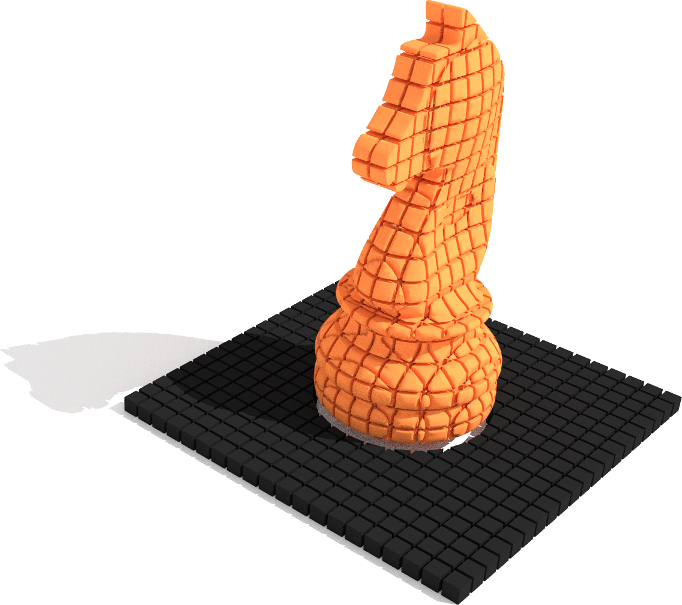
\includegraphics[width=0.35\paperwidth]{side_bar}\\
		\column{0.01\textwidth}
		\column{0.70\textwidth}
			\titlepage
			\hspace*{+0.5em}
			\begin{center}
				
\includegraphics[height=1.0cm]{lidet-logo}\\
				
\includegraphics[height=1.0cm]{ime-logo}\\
			\end{center}
	\end{columns}
	%\addtocounter{framenumber}{-1}
\end{frame}
}

% ---------------------------------------------------------------------------- %
% Other Slides (index from 1 onwards)
% ---------------------------------------------------------------------------- %

% setup navigation symbols and footline
\setbeamertemplate{navigation symbols}{}
\makeatletter
\setbeamertemplate{footline}{%
    \leavevmode%
    \hbox{%
        \begin{beamercolorbox}[wd=0.28\paperwidth,ht=4ex,dp=1ex,left,%
                               leftskip=2ex]{author in head/foot}%
            \usebeamerfont{title in head/foot}
            \insertdate\newline%
            \vskip 0.6ex%
            \autores
        \end{beamercolorbox}%
        \begin{beamercolorbox}[wd=0.53\paperwidth,ht=4ex,dp=1ex,center]%
                              {author in head/foot}%
            \usebeamerfont{author in head/foot}\lessontitle%
        \end{beamercolorbox}%
        \begin{beamercolorbox}[wd=0.19\paperwidth,ht=4ex,dp=1ex,right,%
                               rightskip=2ex]{author in head/foot}%
            \insertframenumber{}/\inserttotalframenumber \newline
            \lidet%
        \end{beamercolorbox}%
    }%
    \vskip 4cm%
}
\makeatother

% ---------------------------------------------------------------------------- %
\begin{frame}[plain]
\frametitle{\textbf{Agenda}}
	\hspace*{+4.0em}
	\footnotesize{ \tableofcontents }
\end{frame}


% ---------------------------------------------------------------------------- %
\section{Mecânicas de jogo}
% ---------------------------------------------------------------------------- %

% MISC:

% Alguns jogos são projetados de modo que o único modo de vencer ou cumprir
% certo objetivo seja fazer exatamente o que o designer quer (como nos puzzles)
% Jogadores são guiados em ``trilhos'' -> tutoriais
% Mas no geral, é interessante ter um conjunto pequeno e bem claro de regras
% mas que permitam ``infinitas'' possibilidades -> comportamento emergente.
% -> Rocket jump

% Regras são escritas no manual. Mecânicas ficam escondidas.

% Mecânicas não dependem de mídia (ou implementação)
% -> Porém a mídia certamente está relacionada com a viabilidade do uso de
%    certas mecânicas.

% Missões -> exercitam o aprendizado das mecânicas
% -> Mate 10 monstros

% Fluxo: Desafio x Habilidade

% Senso de urgência -> motivação

% Progressão

\subsection{O que é mecânica de jogo?}
% ------------------------------
\begin{frame}{\textbf{O que é mecânica de jogo?}}
    \centering
    \begin{itemize}
        \item O baralho é um jogo?
        \pause
        \vskip 1cm%
        \item E poker é um jogo?
    \end{itemize}
\end{frame}

% ------------------------------
\begin{frame}{\textbf{O que é mecânica de jogo?}}
    \centering
    Regras que definem como o jogador e os diversos elementos presentes no jogo
    interagem entre si.
    % -> Adaptação de
    %    Sicart, Miguel. "Defining Game Mechanics",
    %    http://gamestudies.org/0802/articles/sicart
    %    (consultado em 13 de janeiro de 2015)
\end{frame}

% ------------------------------
\begin{frame}{\textbf{Regras}}
% Regras... \cite{Tekinbas2003}
% - Limitam a ação do jogador
% - São explícitas e livres de ambiguidade
% - São compartilhadas por todos os jogadores
% - São fixas
% - Seu cumprimento é obrigatório
% - São reutilizáveis
\end{frame}

% ------------------------------
\begin{frame}{\textbf{Regras em três camadas}}
% Regras em três camadas:\cite{Tekinbas2003}
% - Regras operacionais
%   -> Regras ``escritas''
%   -> Guiam o comportamento do jogador
% - Regras constituintes
%   -> Regras de funcionamento por baixo do pano
%   -> Formalização matemática
%   -> Dois jogos ``diferentes'' podem ter as mesmas regras constituintes (3 to 15)
%   -> São independentes de materiais e até mesmo do jogador
% - Regras implícitas
%   -> Regras não escritas (bom senso)
%   -> Boas práticas, espírito esportivo
\end{frame}

% ------------------------------
\begin{frame}{\textbf{Menos é mais}}
% Nolan's law:
% All the best games are easy to learn and difficult to master. They should reward the first quarter and the hundredth.
% Nolan Bushnell (fundador da Atari)
% - Funciona muito bem para jogos estratégicos e também para jogos de habilidade
% - Go, Xadrez, poker
% - Flappy bird, Super Meetboy, Street Fighter IV
\end{frame}

% ------------------------------
\begin{frame}{\textbf{Sistemas de feedback}}
    % Feedback negativo -> trabalha para atenuar o efeito que tenta despontar.
    %                      Estabiliza o sistema (jogo)
    % Feedback positivo -> amplifica as diferenças
    %                      Favorece o desequilíbrio
\end{frame}


\subsection{Fanstasia integrada à mecânica}
% Fantasia integrada na mecância
% -> The Amazing Spider-Man 2 \url{https://www.youtube.com/watch?v=o9kr9ZhydK0}
% -> Unfinished swan \url{https://www.youtube.com/watch?v=WyFtfvFG4IE}
% -> Amnesia - The Dark Descent /url{https://www.youtube.com/watch?v=JEHPwAvrc_U}
% -> Closure \url{https://www.youtube.com/watch?v=aGRkFT3NHp8}
% -> Ticket to ride \url{http://cf.geekdo-images.com/images/pic2332558_lg.jpg}
% -> Ca$h 'n Gun$ \url{http://cf.geekdo-images.com/images/pic959405_lg.jpg}
% -> Framed \url{https://www.youtube.com/watch?v=jDyC2Ht6pnU}

% Quando a fantasia não se encaixa na mecânica, perde-se imersão.
% -> Mais difícil para o jogador assimilar ações

\subsection{O personagem precisa mesmo morrer?}
% Você precisa mesmo matar o personagem?
% -> Explicação dos arcades
% -> Save points
% -> Time rewind (Prince of Persia) -> jogos de corrida
%    \url{http://i.playground.ru/i/28/78/11/00/blog/icon.600xauto.jpg?v1}


\subsection{Mecânicas e os pilares de motivação}
% ------------------------------
\begin{frame}{\textbf{Mecânicas e os pilares de motivação}}
    \centering
    \begin{minipage}{7cm}
        \begin{description}
            \item[Gameplay:] ações dentro do jogo
            \vskip 1cm%
            \item[Jogabilidade:] capacidade de jogar bem
        \end{description}
    \end{minipage}
\end{frame}


% ------------------------------
\subsection{Exemplos de mecânicas}
    % Exemplos (deturbando a definição inicial)
    % Power-ups
    %   - Pacman
    % Racing games
    %   - Gamão, Jamaica
    % Efeito elástico (catch-up) -> feed back negativo do sistema
    %   - Daytona USA
    % Pontos de experiência -> feedback positivo
    %   - Qualquer RPG basicamente
    %   - Diablo II
    % Worker placement
    %   - Stone Age, Agrícola, Caylus, Age of Empires, Star Craft
    % Coleta de recursos (harvest)
    %   - Stone Age, Agrícola, Caylus, Age of Empires, Star Craft
    % Construção (elementos estáticos, melhorias, unidades) (com gasto de recursos)
    %   - Stone Age, Agrícola, Caylus, Age of Empires, Star Craft
    % Combate de unidades
    %   - Small World, Age of Empires, Star Craft
    % Pedra-papel-tesoura
    %   - Age
    % Árvore de tecnologia/habilidades
    %   - Caylus, Diablo II
    % Set collection
    %   - 7 Wonders, Citadels
    % Interpretação
    %   - Avalon, Spy Party
    % Blefe
    %   - Cash'n Guns
    % Troca
    %   - Settlers of Catan
    % Aposta/leilão
    % Tile placement
    %   - Carcassone
    % Player elimination
    % Drafting
    % Ação simultânea (escolha prévia, revelação simultânea)
    % Controle de área
    % Take that
    % Construção de rotas
    % Rolagem de dados
    %-
    % Portas
    % Blocos empurráveis
    % Interruptores/alavancas
    % Plataformas
    % Esteiras
    % Tranca e fechadura (não precisa ser literal)
    % -> Habilidade/tile que permite gerar construções de um tier acima
    % -> Recursos para passar de idade
    % -> Habilidade de voar/double jump/atirar mais forte...
    % Tempo limitado (não precisa ser literal)
    % -> Bola rolando atrás do personagem
    % -> Porta se fechando lentamente
    % Quebra-cabeça de tempo (espera)


% ------------------------------
\begin{frame}{\textbf{}}
    \centering
    \begin{minipage}{7cm}
        \begin{itemize}
            \item Forma e função
            \vskip 1cm%
            \item Personalidade
        \end{itemize}
    \end{minipage}
\end{frame}


% ---------------------------------------------------------------------------- %
\section{Definição do público-alvo}
% ---------------------------------------------------------------------------- %

% ------------------------------
\begin{frame}{\textbf{Motivação e importância}}

	\begin{outline}

		\1 A experiência é individual e dependente de contexto
			\2[-] {\scriptsize e assim é impossível de garantir!}

		\vspace{1em}

		\1 É difícil fazer testes antes de tomar algumas decisões de projeto
			\2[-] {\scriptsize porque os testadores precisam de algo pra jogar!}

		\vspace{1em}

		\1 As decisões de projeto são sempre direcionadas a jogadores humanos
			\2[-] {\scriptsize afinal jogos são feitos para alguém jogar!}

		\vspace{1em}

		\1 Os projetistas costumam ter ideias vagas ou contraditórias sobre os jogadores
			\2[-] {\scriptsize acabando por se basear em si mesmos e/ou em pessoas muito similares a eles}

	\end{outline}

\end{frame}

% ------------------------------
\begin{frame}{\textbf{Motivação e importância}}

	Deve ser possível perceber algumas dificuldades:

	\vspace{0.5em}

	\begin{outline}
		\1 Dificuldade na identificação e na comunicação das experiências desejadas
			\2[-] {\scriptsize cada projetista, artista, programador, etc pode ter alvos diferentes}
			\2[-] {\scriptsize é um problema grande especialmente em projetos com muitos profissionais}

		\vspace{1em}

		\1 Dificuldade na realização e aproveitamento dos testes de avaliação
			\2[-] {\scriptsize os protótipos iniciais serão provavelmente distantes do desejado}
			\2[-] {\scriptsize é mais difícil obter participantes adequados}
			\2[-] {\scriptsize as avaliações obtidas são menos úteis}
			\2[-] {\scriptsize a equipe pode demorar a perceber o real o público-alvo}
	\end{outline}

\end{frame}

% ------------------------------
\begin{frame}{\textbf{Cartões de personas}}

	Uma técnica bastante útil é chamada de Personas:

	\begin{quotation}
		\noindent
		{\large ``Personas são arquétipos de usuários que representam o público-alvo de um produto.
		Eles são mais bem desenvolvidos em conjunto com a pesquisa de mercado.''\\[0.5em]
		\noindent
		\hfill -- Emily Brown \cite{Brown2010}}
	\end{quotation}

	\cite{Pruitt2003}\\
	
\end{frame}

% ------------------------------
\begin{frame}{\textbf{Adequação às capacidades do público-alvo}}
    \centering
    \begin{minipage}{7cm}
        \begin{description}
            \item[Gameplay:] ações dentro do jogo
            \vskip 1cm%
            \item[Jogabilidade:] capacidade de jogar bem
        \end{description}
    \end{minipage}
\end{frame}


% ---------------------------------------------------------------------------- %
\section{GDD - Game Design Document}
% ---------------------------------------------------------------------------- %
% ------------------------------
\begin{frame}{\textbf{GDD - Game Design Document (Documento de Projeto do Jogo)}}
    \centering
    \begin{minipage}{8cm}
        \begin{itemize}
            \item Documento interno que descreve o jogo
            \vskip 0.4cm%
            \item Não há padrão universal
            \vskip 0.4cm%
            \item Pode ter de 1 a $\infty$ páginas
            \vskip 0.4cm%
            \item Vamos ver hoje uma estrutura recomendável para um documento de
                  10 páginas no máximo
        \end{itemize}
    \end{minipage}
\end{frame}

% ------------------------------
\begin{frame}{\textbf{GDD - Game Design Document (Documento de Projeto do Jogo)}}
    \centering
    \begin{minipage}{5cm}
        Estrutura geral:
        \vskip 0.3cm%
        \begin{enumerate}
            \item Introdução
            \vskip 0.2cm%
            \item Descrição
            \vskip 0.2cm%
            \item Características
            \vskip 0.2cm%
            \item Plataforma(s)
            \vskip 0.2cm%
            \item Concept art\\(arte conceitual)
            \vskip 0.2cm%
            \item Jogos similares
        \end{enumerate}
    \end{minipage}
\end{frame}

% ------------------------------
\begin{frame}{\textbf{GDD - Game Design Document (Documento de Projeto do Jogo)}}
    \centering
    \begin{minipage}{7cm}
        Objetivos:
        \vskip 0.4cm%
        \begin{itemize}
            \item Comunicação
            \vskip 0.4cm%
            \item Compartilhar a mesma visão do jogo entre todos na produção
            \vskip 0.4cm%
            \item Memória
        \end{itemize}
    \end{minipage}
\end{frame}


\subsection{Introdução}
    \begin{frame}{Introdução (ou \textit{Sobre o jogo})}
        Deve descrever o jogo da forma mais concisa possível.

        Precisa deixar explícito:
        \begin{itemize}
            \item Título
            \item Gênero
            \item Plataforma
            \item Objetivo (recomendado, mas opcional)
            \item \textbf{Diferencial}
        \end{itemize}
        \vskip \baselineskip

        Deve ter um ou dois parágrafos, mas precisa instigar curiosidade para o
        leitor querer saber mais sobre o jogo (e jogá-lo!).
        \vskip \baselineskip

        A introdução pode ser vista como o \textit{pitch} do jogo.
    \end{frame}

    \begin{frame}{Importância do título}
        É muito importante escolher bem o título do jogo, pois é ele identidade
        ao produto.
        \vskip \baselineskip

        O título também é um forte elemento de contextualização.
        \vskip \baselineskip

        SEMPRE que for feita referência ao jogo, use o título.

        NUNCA use ``o jogo'', ``nosso jogo'', etc.
    \end{frame}

    \begin{frame}{Exemplos}
        \textbf{Killing Floor}
        \vskip \baselineskip

        \textit{
            Killing Floor é um FPS cooperativo de sobrevivência e terror que se
            passa em cidades e nos campos devastado da Inglaterra depois de que
            uma série de experimentos militares de clonagem dá horrivelmente
            errado. Você e seus amigos são membros de uma equipe militar enviada
            a esses locais com uma missão simples: sobreviver o suficiente para
            limpar a área dos experimentos que falharam.
        }
    \end{frame}

    \begin{frame}{Exemplos}
        \textbf{Chivalry: Medieval Warfare}
        \vskip \baselineskip

        \textit{
            Sitie castelos e invada vilas em Chivalry: Medieval Warfare, um
            slasher em primeira pessoa com foco no muti-player. Com combate
            competitivo on-line que procura capturar a verdadeira experiência de
            estar num campo de batalha medieval. Inspirado na intensidade e
            grandeza de filmes com batalhas de espadas, tais como 300, Gladiador
            e Coração Valente, Chivalry: Medieval Warfare traz essa experiência
            às mãos do jogador.
        }
        \vskip \baselineskip

        \textit{
            O jogo é baseado em habilidade e controles de FPS, mas em vez de
            armas e granadas, o jogadores recebem espadas, escudos, maças,
            machados de batalha e arcos longos. Ambientado em um mundo fictício,
            porém bravo e realista, os jogadores lutarão em batalhas on-line
            frenéticas sitiando castelos, invadindo vilas medievais e lutando
            por glória na arena com até 32 jogadores.
        }
    \end{frame}

    \begin{frame}{Exemplos}
        \textbf{Planetary Annihilation}
        \vskip \baselineskip

        \textit{
            Colonize sistemas solares, aniquile mundos e oblitere seus
            adversários em batalhas interplanetárias épicas com múltiplos
            jogadores e centenas de unidades. Planetary Annihilation leva o RTS
            a uma escala jamais vista - e dá aos jogadores ferramentas poderosas
            para controlar a ação.
        }
        \vskip \baselineskip

        \textit{
            Controle espaçonaves destruidoras, poderosos tanques e uma seleção
            de outras máquinas de guerra futuristas em batalhas épicas através
            de sistemas solares inteiros. Monte planetas inteiros como bases e
            teletransporte suas unidades estrategicamente direto no coração das
            fortalezas de seus inimigos. Ou encerre partidas com a mãe de todas
            as armas: um asteroide em curso de colisão. Não apenas vença,
            aniquile!
        }
    \end{frame}

    \begin{frame}{Exemplos}
        \textbf{The Stanley Parable}
        \vskip \baselineskip

        \textit{
            O Stanley Parable é um jogo de exploração em primeira pessoa. Você
            jogará como Stanley e você não jogará como Stanley. Você seguirá uma
            história, você não seguirá uma história. Você terá uma escolha, você
            não terá escolha. O jogo terminará, o jogo nunca terminará.
            Contradição seguida de contradição, as regras de como o jogo deveria
            funcionar são quebradas e quebradas novamente. Este mundo não foi
            feito para você compreendê-lo.
        }
        \vskip \baselineskip

        \textit{
            Mas à medida que você explora, lentamente, significados começam a
            surgir, os paradoxos podem fazer sentido, talvez você tenha poder
            afinal. O jogo não está aqui para lutar com você; ele convida você
            a dançar.
        }
    \end{frame}


\subsection{Descrição}
    \begin{frame}{Descrição}
        Idealmente com uma ou duas páginas, é o ``miolo'' do GDD.
        \vskip \baselineskip

        Tem como objetivo:
        \begin{itemize}
            \item Mostrar os elementos chave do jogo;
            \item Descrever o contexto e cenário;
            \item Indicar as motivações e/ou objetivos;
            \item Mostrar o que o jogador pode fazer;
            \item Elencar as mecânicas de monetização e socialização\\
                  (se for o caso).
        \end{itemize}
        \vskip \baselineskip

        E o mais importante de tudo...
    \end{frame}

    \begin{frame}{Descrição}
        \centering
        \Large Deixar explícito os\\\textit{fatores de diversão}!
    \end{frame}

    \begin{frame}{Escrevendo}
        Estabeleça uma conversa com o leitor\\
        (leitor = jogador);
        \vskip \baselineskip

        Seja conciso;
        \vskip \baselineskip

        Não coloque ``detalhes de implementação'' nas descrições.
    \end{frame}

    \begin{frame}{Exemplos}
        \begin{block}{Ruim}
            ``O jogador usará as teclas + e - para aumentar ou diminuir o ângulo
            de inclinação do canhão e a força do disparo será proporcional ao
            tempo em que a tecla de espaço permanecerá pressionada.''
        \end{block}
        \vskip \baselineskip

        \begin{block}{Bom}
            ``Você poderá controlar o ângulo de inclinação do canhão e a força
              do disparo para atingir seus inimigos com precisão.''
        \end{block}
    \end{frame}


\subsection{Características} % Key features
    \begin{frame}{Características principais}
        Lista objetiva com características funcionais do jogo.\\
        (Sessão \textit{Key features} dos jogos no Steam)
        \vskip \baselineskip

        Objetivo é destacar rapidamente os elementos...
        \begin{itemize}
            \item inovadores;
            \item muito bons;
            \item que são diferenciais;
            \item que trazem diversão.
        \end{itemize}
    \end{frame}

    \begin{frame}{Características principais}
        Exemplo:
        \begin{itemize}
            \item Mais 8.000 achievements!
            \item Badges colecionáveis;
            \item Física ultra realista;
            \item Fases criadas procedimentalmente;
            \item Inimigos com IA implacável, que aprende com seus erros.
        \end{itemize}
    \end{frame}

    \begin{frame}{Objetivo da lista de características}
        \begin{block}{Nortear o desenvolvimento}
            Essa é a lista de promessas do que haverá no jogo. Portanto, é o
            principal guia do que precisa ser feito.
        \end{block}
        \vskip \baselineskip

        Cada item será um grande objetivo de implementação.\\
        As tarefas serão criadas a partir disso.
        \vskip \baselineskip

        Se alguma tarefa de desenvolvimento não estiver relacionada com nenhum
        item dessa lista, então ela \textbf{NÃO} é importante.
    \end{frame}


\subsection{Plataforma(s)}
    %- Descrever diretamente qual é a plataforma alvo e a forma básica de interação.

    %- Exemplo: PC com teclado e mouse; PC e câmera para captura de movimentos.
    \begin{frame}
        Simplesmente descrever qual é a plataforma alvo e a forma básica de
        interação.
        \vskip \baselineskip

        Exemplo:
        \begin{itemize}
            \item PC (Windows e Linux), com teclado e mouse;
            \item Browser, com mouse ou touch;
        \end{itemize}
        \vskip \baselineskip

        Também nessa seção pode-se colocar a meta de requisitos mínimos que
        deseja-se atingir.
        \vskip \baselineskip

        OBS: idealmente, deveria-se ter ideia do público alvo também.

    \end{frame}


\subsection{Concept art}
    \begin{frame}{Concept art}
        Deve conter as ilustrações para exemplificar cenários, personagens,
        objetos, itens coletáveis, etc.
        \vskip \baselineskip

        Outros elementos visuais, como tela inicial, HUD, menus também podem ser
        colocados aqui.
        \vskip \baselineskip

        Todas as ilustrações podem ser apenas esboços.\\
        (Vale mais ter 10 esboços diferentes do que 1 arte-final)
        \vskip \baselineskip

        Também é valido colocar fotos de locais, veículos ou mesmo elementos de
        outros jogos para servirem de \textbf{referência}.
    \end{frame}

    \begin{frame}{Importância do cocept art}
        Mesmo sem a arte final, pelo concept já é possível entender o estilo e o
        clima que o jogo terá. \\
        (Sombrio, cartunesco, colorido, realista, etc.)
        \vskip \baselineskip

        Ajuda fortemente o compartilhamento de uma \textbf{visão única} do jogo
        entre todos os envolvidos no projeto.
    \end{frame}


\subsection{Jogos similares}
    \begin{frame}{Jogos similares (opcional)}
        Todo esforço para favorecer a \textbf{visão única} sobre o jogo é
        válido.
        \vskip \baselineskip

        Assim, é importante listar quais jogos tem mecânica, temática ou arte
        parecida com a que se deseja fazer.
        \vskip 4\baselineskip

        OBS: Além disso é importante tentar descobrir se um jogo igual ou muito
             parecido já existe.
    \end{frame}

    \begin{frame}{Exemplos de GDD}
        \centering
        Vamos ver dois exemplos de documentos...
    \end{frame}


% ---------------------------------------------------------------------------- %
\section{Atividade}
% ---------------------------------------------------------------------------- %

% ------------------------------
\begin{frame}{Atividade}
    \centering
    \begin{minipage}{9cm}
        \begin{itemize}
            \item Definir público alvo e montar personas
            \vskip 0.6cm%
            \item Definir (ou melhorar) as mecânicas do projeto
            \vskip 0.6cm%
            \item Mater a coerência com os pilares da motivação\\
                  \textit{(Justificar escolhas, impacto no gameplay e relação
                  com as personas)}
            \vskip 0.6cm%
            \item Elaborar um GDD
        \end{itemize}
	\end{minipage}
\end{frame}

% ------------------------------------------
% References
% ------------------------------------------

\referencesbegin
\begin{frame}[plain, allowframebreaks]
	\frametitle{\textbf{References}}
	\bibliographystyle{abbrv}
	{\tiny \bibliography{bibliography}}
\end{frame}
\referencesend


\end{document}

